\documentclass[spanish,a4paper,11pt]{article}
\usepackage{graphicx}
\usepackage{float}
\usepackage[export]{adjustbox}
\usepackage[affil-it]{authblk}
\usepackage[utf8]{inputenc}
\usepackage[spanish]{babel}
\usepackage{siunitx}
\setlength{\parskip}{2mm} % {6mm}
\usepackage{derivative}
\usepackage[margin=2.5cm]{geometry}
\usepackage{amsmath}
\usepackage{amssymb}
\usepackage{svg}
\usepackage[font={footnotesize}, labelfont=bf]{caption}
\usepackage{subcaption}
\usepackage{chngcntr}
\makeatletter
\newcommand*{\centerfloat}{%
  \parindent \z@
  \leftskip \z@ \@plus 1fil \@minus \textwidth
  \rightskip\leftskip
  \parfillskip \z@skip}
\makeatother
\counterwithin{figure}{section}
\counterwithin{table}{section}
\counterwithin{equation}{section}

\usepackage{geometry}
\usepackage{fancyhdr}
\usepackage[dvipsnames]{xcolor}
\usepackage{appendix}
\usepackage{subcaption}
\usepackage{multirow}
\usepackage{longtable}
\usepackage[font=footnotesize, labelfont=bf, width=0.8\textwidth, justification=justified]{caption}
\usepackage[pdfencoding=auto, psdextra]{hyperref}
\usepackage{titlesec}
\usepackage{csquotes}
\usepackage[backend = biber,sorting = none]{biblatex}
\usepackage{listings}
\usepackage{xcolor}

\definecolor{codegreen}{rgb}{0,0.6,0}
\definecolor{codegray}{rgb}{0.5,0.5,0.5}
\definecolor{codepurple}{rgb}{0.58,0,0.82}
\definecolor{backcolour}{rgb}{0.95,0.95,0.92}

% --- MODIFICADO AQUÍ ---
\lstdefinestyle{mystyle}{
	backgroundcolor=\color{backcolour},   
	commentstyle=\color{codegreen},
	keywordstyle=\color{magenta},
	numberstyle=\tiny\color{codegray},
	stringstyle=\color{codepurple},
	basicstyle=\ttfamily\footnotesize,
	breakatwhitespace=false,         
	breaklines=true,                 
	captionpos=b,                    
	keepspaces=true,                 
	numbers=left,                    
	numbersep=5pt,                   
	showspaces=false,                
	showstringspaces=false,
	showtabs=false,                  
	tabsize=2,
	% --- LÍNEA AÑADIDA PARA UTF-8 EN LISTINGS ---
	literate={á}{{\'a}}1 {é}{{\'e}}1 {í}{{\'i}}1 {ó}{{\'o}}1 {ú}{{\'u}}1 {Ñ}{{\~N}}1 {ñ}{{\~n}}1
}
% --- FIN DE LA MODIFICACIÓN ---

\lstset{style=mystyle}
\addbibresource{Referencias.bib}
\fancyhf{}
\fancyhf{}
\rhead{}
\lhead{Universidad de Buenos Aires - FCEN}
\rfoot{\thepage}

\begin{document}
\renewcommand{\listtablename}{Índice de tablas}
\renewcommand{\tablename}{Tabla}


\begin{center}
    {\LARGE
    \textbf{Mapas y Asimetrías Azimutales de la Densidad de Muones de Lluvias Atmosféricas Extensas con el Detector Subterráneo de Muones del Observatorio Pierre Auger}}

    \vspace{1cm}
    
    \large\textbf{Notas sobre la Tesis}

    \vspace{1cm}

    \textbf{Lautaro Silva} \\
    Mail: lautarosilvapizzi@gmail.com \\
    DNI: 43441919 \\
    LU: 879/21 \\

    \vspace{0.5cm}

    \textit{ITeDA - CAC - CNEA \\
    Depto. de Física - FCEyN - UBA}
        
    \vspace{0.5cm}
        
    Septiembre 2025
\end{center}


\section{Notas sobre los papers}
\subsection{GAP-1998 Auger project technical note. Asymmetry of Air Showers at Ground Level \cite{paper_1998}}

La pregunta central sobre lo que se va a trabajar es si es cierto (que sabemos que no) la afirmación que dice Pryke sobre:

“It is frequently assumed that the signals observed when an extensive air shower strikes a ground array depend only on perpendicular distance from the shower axis (core distance)”

$\Rightarrow$ Las primeras cosas que propone es que:

\begin{itemize}
    \item Para eventos muy angulares no sucede que solo depende de la distancia porque al atravesar mas aire se siguen desarrollando aun mas las lluvias (“due to continuing longitudinal development of the cascade”).
    \item Y después habla de lo mas importante que es el hecho de que el efecto del campo geomagnético distorsiona aun en las lluvias mas perpendiculares.
\end{itemize}

Pryke va a mostrar que el efecto geomagnético es predominante en lluvias de $E \geq 10^{19}$eV y $\theta \leq 60^\circ$

$\underline{def:}$ impact parameter: distancia radial respecto al eje en el plano de la lluvia (recordar que esto se proyecta de manera “elíptica” sobre la superficie)

Algo obvio es que: “In fact for non vertical showers (…) as the cascade continues to develop (…) the particles which strike the ground first represent an earlier stage of development than those which arrive later”.

\colorbox{yellow}{
  \parbox{\dimexpr\textwidth-2\fboxsep}{%
  PREGUNTA: actualmente se sigue midiendo solo hasta los $60^\circ$?}}

\colorbox{yellow}{
  \parbox{\dimexpr\textwidth-2\fboxsep}{%
  PREGUNTA: “In fact an air shower cascade disk first grows and then contracts as it passes down through the atmosphere. Ground level is normally beyond the point of maximum development” $\rightarrow$ esto es así??? súper anti-intuitivo
}}

\colorbox{orange}{
  \parbox{\dimexpr\textwidth-2\fboxsep}{%
  RESPUESTA: Actually no, es súper intuitivo, llega un punto donde alcanzan el threshold mínimo para la creación de nuevas partículas y ese es cuando se llega al $X_max$ y ahí solo queda que las partículas de la lluvia choquen y pierdan energía o sean absorbidas por otras de la atmósfera.
}}

Los plots de la Fig 4 parecen razonables (los entiendo), pero los de las Figs 5 y 6 son raros. Lo que entiendo que debería pasar es que a medida que me alejo del eje de la lluvia la proporción de muones tardíos (que se desarrollan mas?) es grande comparado con los tempranos (no termino de entender que quiere decir que podes comparar los tempranos con los tardíos si todos deberían tardar lo mismo en llegar). 

\colorbox{yellow}{
  \parbox{\dimexpr\textwidth-2\fboxsep}{%
  PREGUNTA: como corno llega a decir que lo que espera ver en las distribuciones de partículas (cuando el efecto geomagnético esta apagado) que el efecto de la asimetría temprano-tardía es un primer armónico (sinusoidal?) con supresión en deg=0 y amplificación en $\pm 180^\circ$. (PREGUNTAS NO MUY RELEVANTES)}}

Creo que entendí que es lo que dice $\rightarrow$ vas a ver que el efecto es chico si angularmente estas shallow, ahora, por que es sinusoidal no se?????

Comentario de Juan: este efecto podría no ser tan evidente u observable whatsoever. Esto ya lo dice Pryke, pero no entiendo bien xq. Es por el hecho que el lower limit de la energía necesaria para que los muones decaigan en otras cosas y por ende sigan desarrollándose es grande, entonces llega un punto en el q ya tienen energía por debajo de esto y ya no les da para seguir interactuando entonces siguen de largo. Hipótesis DISCUTIR

Empece a entender un poco el efecto del campo geomagnético (ECG lo voy a llamar por paja de escribir). Te splitea las partículas de carga + y – entonces tenes como dos distribuciones separadas en función de que tanto de modifica el centro.

\colorbox{yellow}{
  \parbox{\dimexpr\textwidth-2\fboxsep}{%
  PREGUNTA: hay efectivamente una diferencia de la carga total de los muones + con – (igual entiendo que no es fácilmente medible la carga de la partícula con los detectores $\rightarrow$ Pryke dice que con los Cherenkov seguro q no y entiendo que con AMIGA tampoco). (PREGUNTAS NO MUY RELEVANTES)}}

Esta conclusión es interesante y piola (asumo que se refiere al valor medio de la distribución porque el ancho debería aumentar): “Hence although the existence of the geomagnetic field may distort the muon charge ratio in the left and right regions the overall muon density is not greatly altered”

\colorbox{yellow}{
  \parbox{\dimexpr\textwidth-2\fboxsep}{%
    PREGUNTA: en el anexo dice devuelta que puede fittear el efecto del ECG como un segundo armónico (dos picos?), why?? (PREGUNTAS NO MUY RELEVANTES)}}


No entendí la ultima frase del paper: “For scintillator detectors the asymmetry would be larger still since they are more reliant on the rapidly attenuating electromagnetic component”.


\subsection{GAP-2002 Towards Parametrization of the Lateral Distribution Function and its Asymmetries in the Surface Detector\cite{paper_2002}}


$\underline{def:}$ Lateral Distribution Function (LDF) is the function that describes empirically the dependence of the signal on the position of the tank with respect to the shower core → is a function of the distance to the core r and of the azimuthal direction (because anisotropies: forward-backward asymmetry and magnetic distortion)

Estoy empezando a preguntarme como es que puedo realizar los mapas de muones en el plano perpendicular a las lluvias, si lo que yo tengo es solamente los detectores subterráneos. La idea es que usando la diferencia temporal entre las detecciones de los diferentes detectores puedo rearmar las lluvias en el plano perpendicular, ponele que te creo eso, pero como hago para extrapolar para atrás en el tiempo como se veían las distribuciones de muones? Es medio raro, no lo entiendo bien. Creo que igual lo que voy a hacer es hacer los mapas sobre la superficie.

Intentando parametrizar esta LDF llegan a una serie de conclusiones:

\begin{itemize}
    \item Para $\theta$ pequeño, la componente electromagnética de la lluvia iniciada por un primario protón, no alcanzo su máximo todavía, frente a lluvias de primarios mas pesados donde la lluvia se ve mas avanzada (‘‘envejecida’’).
    \item Para $\theta$ grande, este efecto es al revés donde las lluvias pesadas son mas avanzadas en su decaimiento que las livianas (protones), pero esto se compensa con la mayor parte muonica de la lluvia que domina para $\theta$ grande
\end{itemize}

Hace un comentario que me pareció relevante para discutir. Dice que las lluvias mas verticales pueden no llegar a ser las mas optimas para la discriminación y que las mejores son las de entre $40^\circ$ y $50^\circ$ donde el "ratio entre tamaño-de-tierra (entiendo que se refiere al detector) / energía es mas favorable". No termino de entender si esto tiene que ver con el hecho de que así   garantizas que las lluvias puedan llegar su $X_{max}$ siempre, pero sin irte a lluvias muy angulares y por ende deformadas ?? Pero no se.

El capitulo 5 es el mas interesante. Habla de varias cosas que creo relevante ir comentando. Primero dice que se va a intentar fittear la asimetría en la detección sobre la superficie como 

\begin{equation}
    S(r,\psi) = \hat{S} (1 + A(r) cos(\psi))
    \label{eq_de_asimetrias}
\end{equation}

Dice que el valor de A desaparece en r=0 lo cual es razonable, porque  sobre el eje no se deforma. Pero después dice algo medio raro, que el valor de A llega a un plateau pero que esto solo lo logran describir empíricamente y no teóricamente (no hay explicación? dice algo como que el problema es que para r grande no hay suficiente estadística). 

Spoiler, yo voy a buscar parametrizar A con no solo la distancia al eje r, sino también con el angulo zenital con el que entra $\theta$.

Una vez q llegan a una parametrizacion dicen esto: "the combination of shower-to-shower variations and satistical fluctuations of the signal in the tank are not negligeble compared to the amplitude of the asymmetry, then a more precise parametrizaction would not really help".

NO ESTOY SEGURO, PERO SUENA Q MANDARON CUALCA

No termino de entender estas frases que dice todo el tiempo de que hay veces que domina la parte muonica.

\subsection{GAP-2022 Extensive air shower asymmetry and
cosmic ray mass composition with the
upgraded Pierre Auger Observatory\cite{tesis_bradfield}}

Frase que me gusta mucho para tener noción de lo raros que son los eventos de alta energía: 

‘‘For comparison, a flux of 1 $particle/m^2/second$ above $10^{14} eV$ drops to approximately 1 $particle/km^2/century$ above $10^{20} eV$.’’

No tiene que ver directamente con la tesis, pero hay varias cosas interesantes que no me había puesto a pensar antes y que son respuestas a preguntas que no me había hecho, por ejemplo por que las UHECR son extra-galácticos: 

“One piece of information the Hillas criterion does allow us to infer is that the lack of measured galactic-plane anisotropy (see Section 1.6) indicates that cosmic rays of the highest energies come from sources which are extra-galactic, such as AGN. This is because protons accelerated to $10^{20}$ eV by a galactic source would have a gyro radius of $\approx$ 100 kpc within the galaxy. This is considerably larger than the radius of the Milky Way at $\approx$ 16 kpc. Therefore, these protons would be expected to travel in nearly straight lines towards Earth, creating a clear hotspot. Since no evidence of such an excess has been observed, the sources for such particles are assumed to be located outside our galaxy”.

Otra cosa mas respecto a las explicaciones de del cutoff de energía a partir de los $10^{19} eV$ que se ve en la Figura puede atribuirse a una de dos cosas (yo entendía que estaba medianamente aceptado que esta asociado al GZK?):

\begin{figure}[!ht]
    \centering
    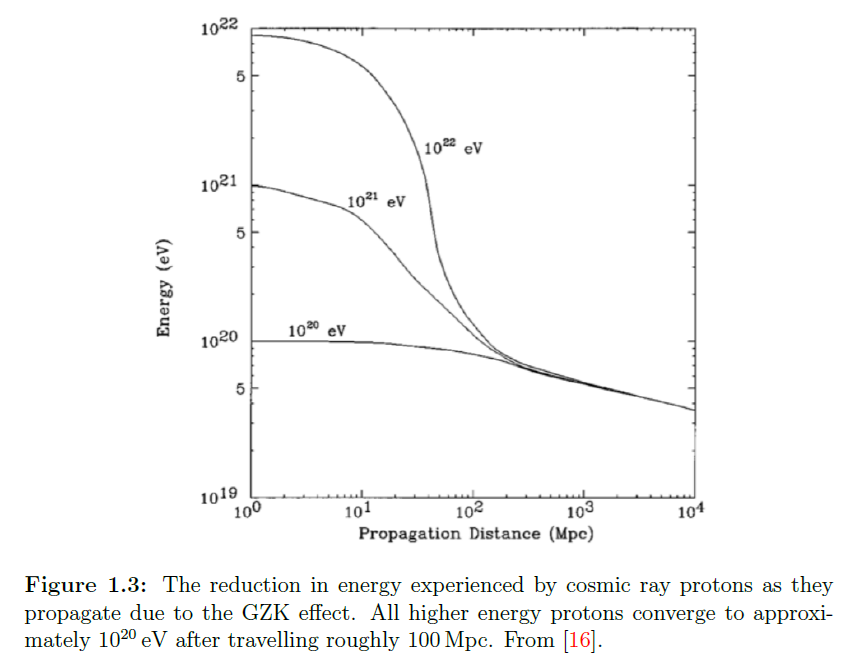
\includegraphics[width=1\linewidth]{Notas Iniciales/GZK.png}
    \label{fig:GZK}
\end{figure}


‘‘As shown in Figure 1.3, these interactions would cause a rapid decrease in energy for any cosmic ray with $E > 10^{20} eV$. This creates a cutoff where, after $\approx 100Mpc$,
any higher energy cosmic ray will converge to $E \approx 10^{20} eV$. An alternative, albeit far less interesting, explanation for the suppression is that sources of cosmic rays cannot accelerate particles to higher energies [15].’’

Otra mas respecto a como es la medición de los primarios en eventos de alta energía donde se usan las EAS:

“(...) the fuctuations in the development of EASs do not allow for the primary composition to be determined on an event by event basis. However by looking at ensembles of showers and their average properties one can estimate the abundance of primaries in 4 mass groups, namely protons (hydrogen), helium, nitrogen and iron. At the highest energies, this is typically done using a shower parameter known as $X_{max}$ essentially a measure of
where in a shower's development the greatest number of particles is observed. The key point is that the $X_{max}$ distributions of lighter primaries, such as proton, have both larger means and standard deviations than heavier primaries like iron. Figure 1.8 shows measurements of the mean and standard deviation of $X_{max}$ distributions as a function of energy from the Pierre Auger Observatory. The lines plotted indicate
predictions based on various hadronic interaction models. When compared with the models, there is a clear change in behaviour around the ankle region, where the
average composition begins to become heavier”.

\begin{figure}[!ht]
    \centering
    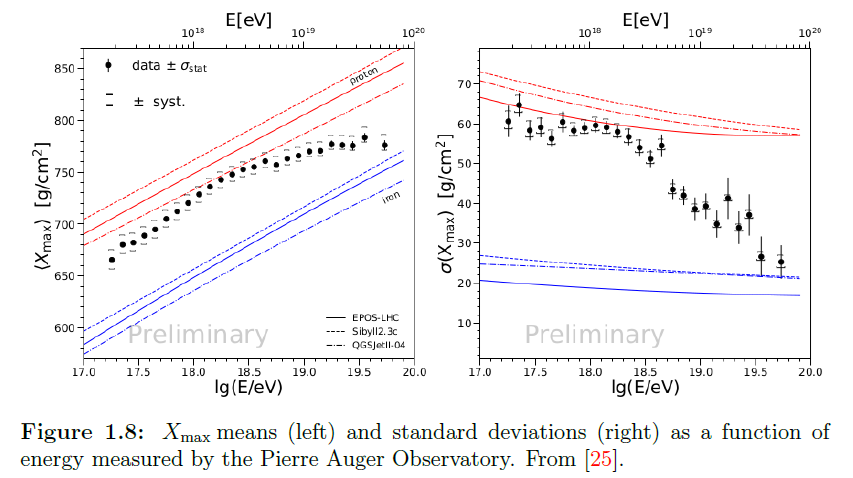
\includegraphics[width=1\linewidth]{Notas Iniciales/X_max_para_light_y_heavy.png}
    \label{fig:X_max}
\end{figure}

Para entender, en el mapa de cielo, cuando se ve que no son isotropicas los UHECR que es ese dipolo del cual se habla? Es la galaxia esta Centauri que menciono el flaco de IB en la charla de la RAFA?

\colorbox{yellow}{
  \parbox{\dimexpr\textwidth-2\fboxsep}{%
    PREGUNTA: Leyendo esto me acorde de una de las preguntas que me hizo Pedro en la RAFA, no sucede en UMD que tenes dos impactos de muones en el tiempo en el que la electrónica responde, mezclándote así las señales de dos eventos diferentes? Es simplemente que esto es improbable por la cantidad de eventos o por la velocidad de respuesta de la electrónica?
}}

\colorbox{orange}{
  \parbox{\dimexpr\textwidth-2\fboxsep}{%
    RESPUESTA: Si pero se logran eliminar con estadística (esta cuantificado cuanto es que pasa y entiendo que es como que lo ‘‘restas’’).
}}

Primer resultado importante que voy a ver si logro replicar respecto a los resultados de la asimetría (entiendo que el parámetro $b$ es el que yo llamo $A$) es: 

‘‘From this plot, we see a clear increase in the magnitude of the asymmetry with zenith angle (in both detectors) for both proton and iron primaries up to the second to last bin, which corresponds to $\approx 50^\circ $. The noticable drop in the asymmetry amplitude in the final bin for each primary/detector type is possibly due to these showers ‘‘running out’’ of electromagnetic particles, which are generally considered to be the primary cause of asymmetry. This may be because of the large amount of atmospheric depth needed to be traversed at large zenith angles. (...) it is evident that the asymmetry is somewhat
greater when measuring showers initiated by proton primaries than iron primaries for zenith angles $\gtrsim 30^\circ ~~(sin^2(\theta) \gtrsim 0.3)$. Again this is probably because of muons,
specically that they constitute a larger portion of the total number of particles in
an iron shower than a proton shower.’’

\begin{figure}[!ht]
    \centering
    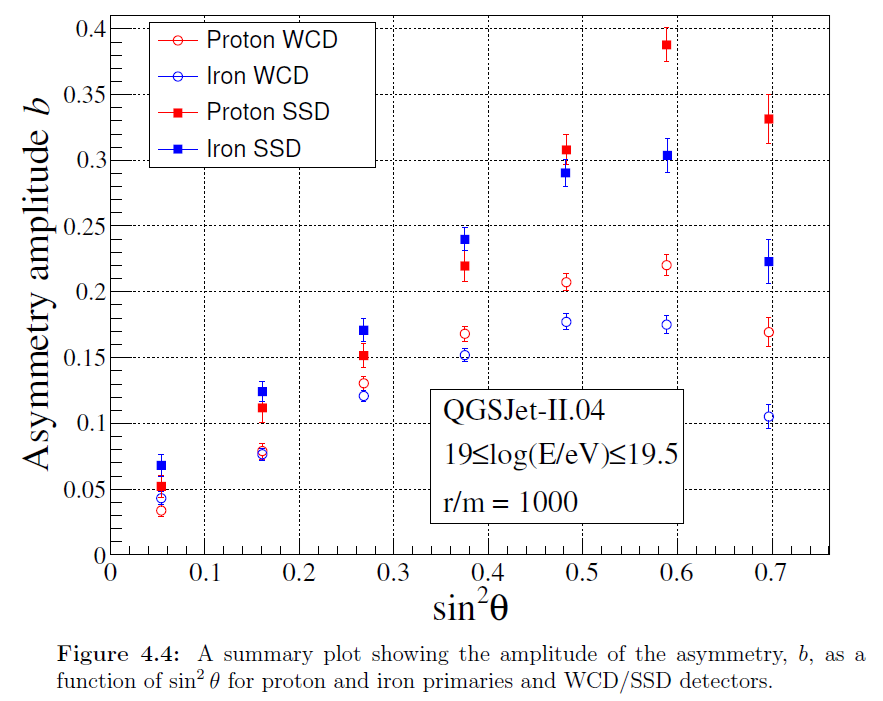
\includegraphics[width=1\linewidth]{Notas Iniciales/asymmetry_amplitude.png}
    \label{fig:asymmetry_amplitude}
\end{figure}

Hay constantemente todo a lo largo de la tesis y de los otros papers frases como estas ‘‘(...) muons, which typically show less asymmetry than electromagnetic particles (...)’’ pero no entiendo por que. Esto lo quiero discutir. Entiendo un poco la razón pero se engancha con las preguntas de antes de que quiere decir que las lluvias se convierten en muónicas y lalala.

Una vez que caracterizo la asimetria comparando lluvias de protones e hierros agarra y se fija cuando son maximas y llega a esto: ‘‘This seems to suggest the maximum difference does not depend significantly on the radius, only on the zenith angle and $log(S_{1000})$.’’€€€¦€€€€€€¦¦¦¦€\\\\\\
\label{sec:Notas_iniciales}
\section{Trabajo - Análisis de datos y Programación}
Es  imperativo para todo el trabajo que estoy haciendo aprender y entender como se ordenan y guardan las cosas en los ADST y en pos de esto, es clave la documentación que se encuentra en: \url{https://web.iap.kit.edu/augeroracle-doc/ADST/html/classes.html}.

A día 9/10/2025 ya va encaminado la lectura de los 600 ADST que me paso Marina y empece a hacer algo de análisis respecto a lo que quiero analizar, pero me falta formalizarlo.

Papers posibles que quiero leer:
\begin{itemize}
    \item \url{https://pure.rug.nl/ws/portalfiles/portal/1243882867/ICRC2023_248.pdf}
    \item \url{https://www.sciencedirect.com/science/article/abs/pii/S0168900207014106?via%3Dihub}
    \item \url{https://link.springer.com/article/10.1140/epjc/s10052-024-13560-5}
    \item \url{https://arxiv.org/pdf/1208.2154}
\end{itemize}

Después de una semana de no hacer nada, hoy 21/10 vamos con una de las cosas que considero que son fundamentales: la limpieza de los datos para las lluvias simuladas. Para esto considero que hay que establecer algunos criterios; tengo algunas propuestas:

\begin{itemize}
	\item Considerar como es la relación entre los valores de $\theta$ y $\phi$ entre la reconstrucción y los valores de la simulación. Establecer un \textit{threshold} para que por encima de cierta diferencia entre estos valores angulares desestimo el \textit{datapoint}. No considero la reconstrucción de la energía porque en general le pega (podría poner algún if para que me diga si no le pega por mucho).
	\item Al final son todos razonables y no hay casi problemas con nada, lo único que a veces la $E_{REC}$ es o 0 o negativa entonces me queda un  -inf pero lo tiro convirtiéndolo en nan's y tirando esas filas.
\end{itemize}

Por otro lado todavía tengo problemas para hacer los plots que yo quiero. Me lo imagino como un plot en polares visto desde arriba donde veo como están distribuidos angularmente en $\theta$ alrededor del eje $z$ pero como q quiero q el radio vaya desde -1 en adelante así no tengo las curvas todas pegadas en cero.

---

Estamos a 30/10, lo de los últimos días fueron todo medio boludeces porque todavía se estaban copiando los datos de los ADST del ruso y los datos de Carmi. Vamos paso a paso, ya revise los tamaños de los ADST y no son tan grandes, son del orden de 10Gb cada uno así que se pueden leer normalmente y sin problemas. Por el lado de los datos de Carmi, el problema es que no tiene el $\varphi$ que es lo que a mi me interesa para hacer los mapas de muones y el análisis de las asimetrías. Entonces, por ahora eso queda descartado.

Vamos ahora con lo que estuve haciendo adaptando mi código para leer los ADST grandes (que igual no debería ser tan un problema ahora). Ya me arme todo el código, despues relleno esto y explico como es q funciona que guardo y lalala. (lo voy a hacer ahora, unas hora despues jeje).

\begin{itemize}
	\item La idea es que hago un loop paralelizado (por ahora 4 workers) sobre los ADST que pesan $\approx 10$Gb y corren cada uno en unos 6.5mín y se guardan en archivos \lstinline|.parquet| de menos de 1Mb c/u. 
	\item  Lo que estoy guardando por ahora es: el id del evento (o lluvia); las energías, $\varphi$ y $\theta$ de MC y REC; el nombre del primario; cantidad de muones; posiciones x-y de los detectores en el plano de la lluvia; distancia r al eje de la lluvia y la posición $\phi$ en polares; y después algunas cositas más

	
		\begin{lstlisting}[language=Python, caption=Generador de SPE]
data.append({
	"event_id": event_id_lluvia, # El ID único de la lluvia
		
	# Info MC
	"logE_MC": logE_MC, "theta_MC": theta_MC, "phi_MC": phi_MC, "primary": primary,
		
	# Info REC
	"logE_REC": logE_REC, "theta_REC": theta_REC, "phi_REC": phi_REC,
		
	# Info específica del Counter
	"counterId": counter.GetId(),
	"nMuones": nMuones,
	"x_plane": x_plane,
	"y_plane": y_plane,
	"phi_plane": phi_plane, # <-- AÑADIDO
	"r_core": r_core,
	"sdId": sdId,
	"sdSignal": sdSignal
})	
\end{lstlisting}

	\item Las 20 simulaciones por energía por modelo por primario de 1200 lluvias c/u con una distribución uniforme de ángulos en $\sin^2(\theta)$ tarda del orden de 40mín.
\end{itemize}

Pero ahora quiero ir a cosas importantes que tengo que ver/leer/discutir:

\begin{itemize}
	\item Ver si haciendo cortes a $r$ fijo se ve alguna cosa característica sobre como es la distribución en función del $\varphi$.
	\item Ver si haciendo estos mismo plot pero con el SD (para esto tengo que cambiar lo que estoy levantando de los ADST) se ve mejor la asimetría mirando solo los muones y si el problema es cuando se lleva al UMD enterrado, en el que sobreviven solo los de alta energía.
	\item Leer del paper de Bradfield (o el de 2002??) si hacia las simulaciones con el offline o solo con CORSIKA.
	\item Ver si el bineado en $r$ tiene sentido hacerlo que scalee con la distancia, es decir, bines más chicos para $r$ más chico (al menos eso entendí de lo que discutí con Fede).
\end{itemize}

---

Indiferentemente de esto, yo ya logre hacer el análisis y levantar al menos a groso modo (o primera iteración) los datos de los ADST de \textbf{Helio con Sibyl de $10^{17.5-18}eV$}.

Hoy estamos a 04/11, voy a contar un poco lo que hice los últimos días. Estuve trabajando en comenzar a hacer el análisis de los datos de los ADST de Alexey de Helio-Sib-$10^{17.5-18}$eV. 

Lo que hice es esencialmente plotear los datos de un solo ADST en 3D donde veo la cantidad de muones en función del angulo polar con el que entraron y la distancia al core. Hasta ahí se veis razonable los resultados que estaba viendo.

Hice el análisis de como se comportaban los datos de manera global, viendo:

\begin{itemize}
	\item Relación entre la $E_{MC}$ y $E_{REC}$ donde se ve que anda mayoritariamente bien pero con una consistente subestima la energía por aproximadamente 0.2 ordenes de magnitud. 
	\item Por el lado de los $\theta$ y $\phi$ no hay mayores problemas y anda re bien.
\end{itemize}

Finalmente hice los mapas polares pero esto es más visual que otra cosa, no sirve mucho para ver efectivamente la asimetría, para eso debería hacer cortes a r fijo.

Hice esto mismo para todos los ADST juntos y se ve el mismo comportamiento con todo (con mayores errores en las reconstrucciones de la energia para eventos de mayor energía, pero son pocos, del orden de 50 teniendo 200k).

Hice lo que creo que es lo que tengo que hacer, que es, agarra mis datos, binearlos en $\theta$ y en $r_{core}$ y plotear cantidad en funcion de $\phi$ de las estaciones donde deberia ver la asimetria. Esto no lo logre, lo cual es una cagada y no me queda claro si estoy haciendo algo mal, o por que no se ve lo que espero.




\textit{NOTAS:} voy a hacer un mini resumen los datos (ADST de Alexey) a los que tengo acceso actualmente (04/11):

\begin{itemize}
	\item Sibyl (modelo hadrónico)
	\begin{itemize}
		\item Energías = $10^{17.5-18}\,\text{eV}$
		\begin{itemize}
			\item Helio ×20
			\item Hierro ×20
			\item Oxígeno ×20
			\item Protones (pero no tengo acceso)
		\end{itemize}
		\item Energías = $10^{18-18.5}\,\text{eV}$ (pero no tengo acceso)
	\end{itemize}
	\item QGS (modelo hadrónico)
	\begin{itemize}
		\item Energías = $10^{17.5-18}\,\text{eV}$
		\begin{itemize}
			\item Helio ×20
			\item Hierro (pero vacío)
		\end{itemize}
		\item Energías = $10^{18-18.5}\,\text{eV}$ (pero no tengo acceso)
	\end{itemize}
	\item EPOSLHC (modelo hadrónico)
	\begin{itemize}
		\item Energías = $10^{17.5-18}\,\text{eV}$
		\begin{itemize}
			\item Helio ×2 (raro)
		\end{itemize}
		\item Energías = $10^{18-18.5}\,\text{eV}$ (pero no tengo acceso)
	\end{itemize}
\end{itemize}

\label{sec:Trabajo_Programacion}

\printbibliography[]
\addcontentsline{toc}{section}{Referencias}

\end{document}
